\section{Experimental Results \label{sec:evaluation}}

\begin{figure*}[t!]
\centering
\subfigure[Attention Aggregation]{
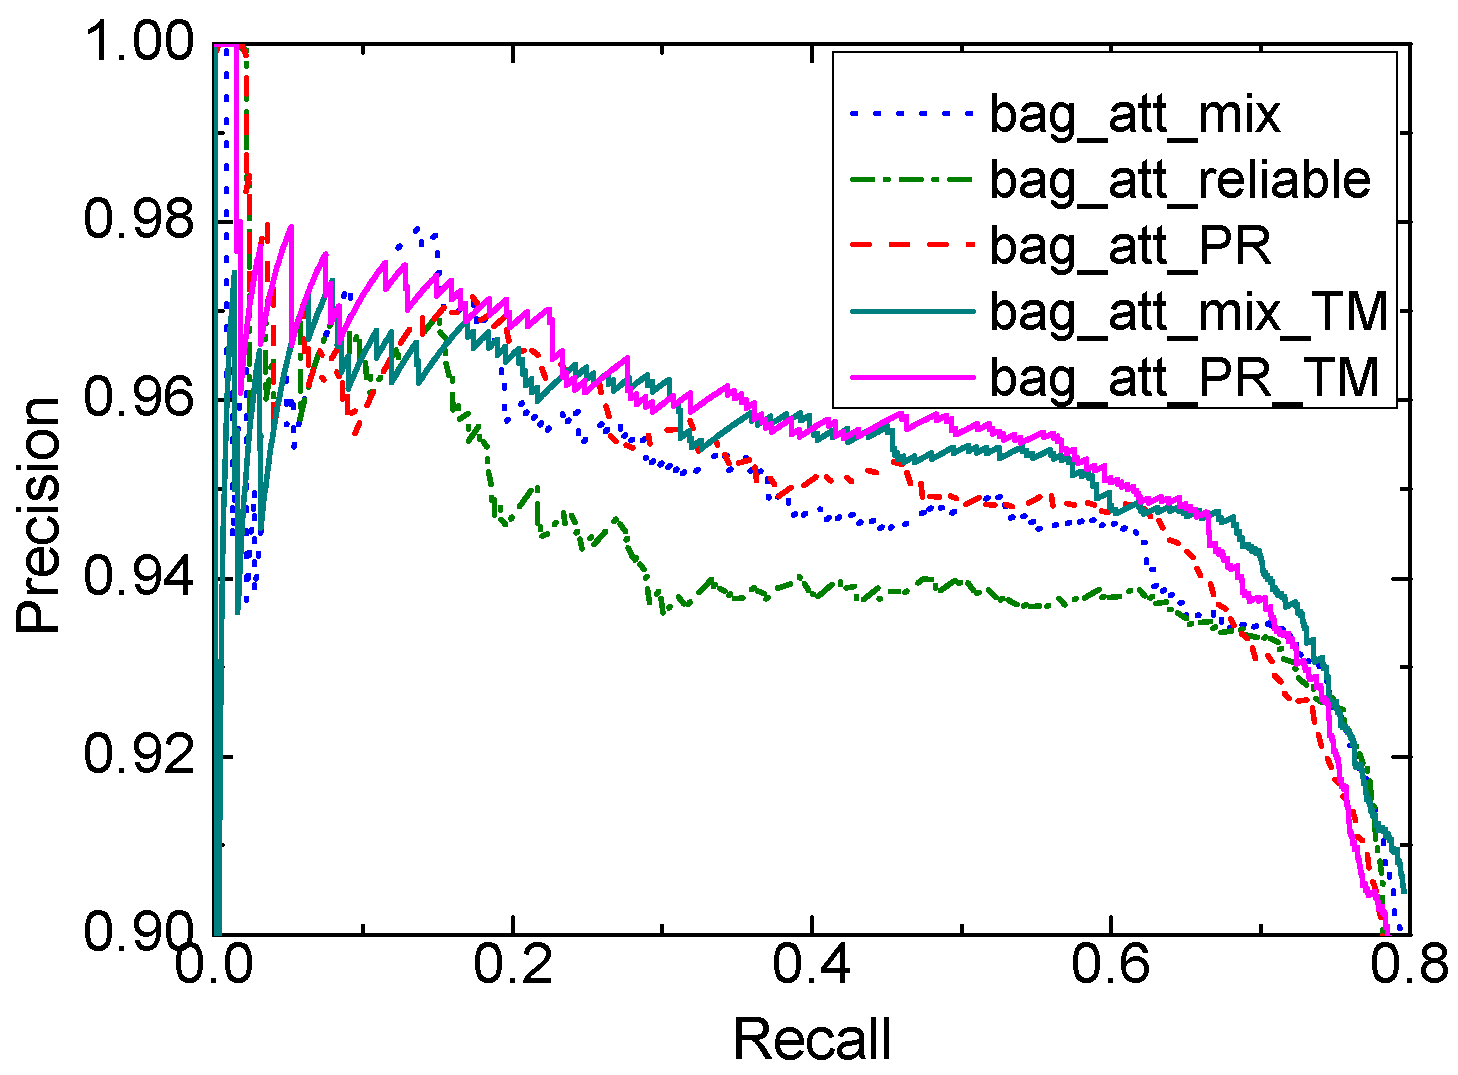
\includegraphics[width=0.48\textwidth]{figures/bag_att_exp_overall.pdf}
\label{fig: bag_att_luo}
}
\subfigure[Average Aggregation]{
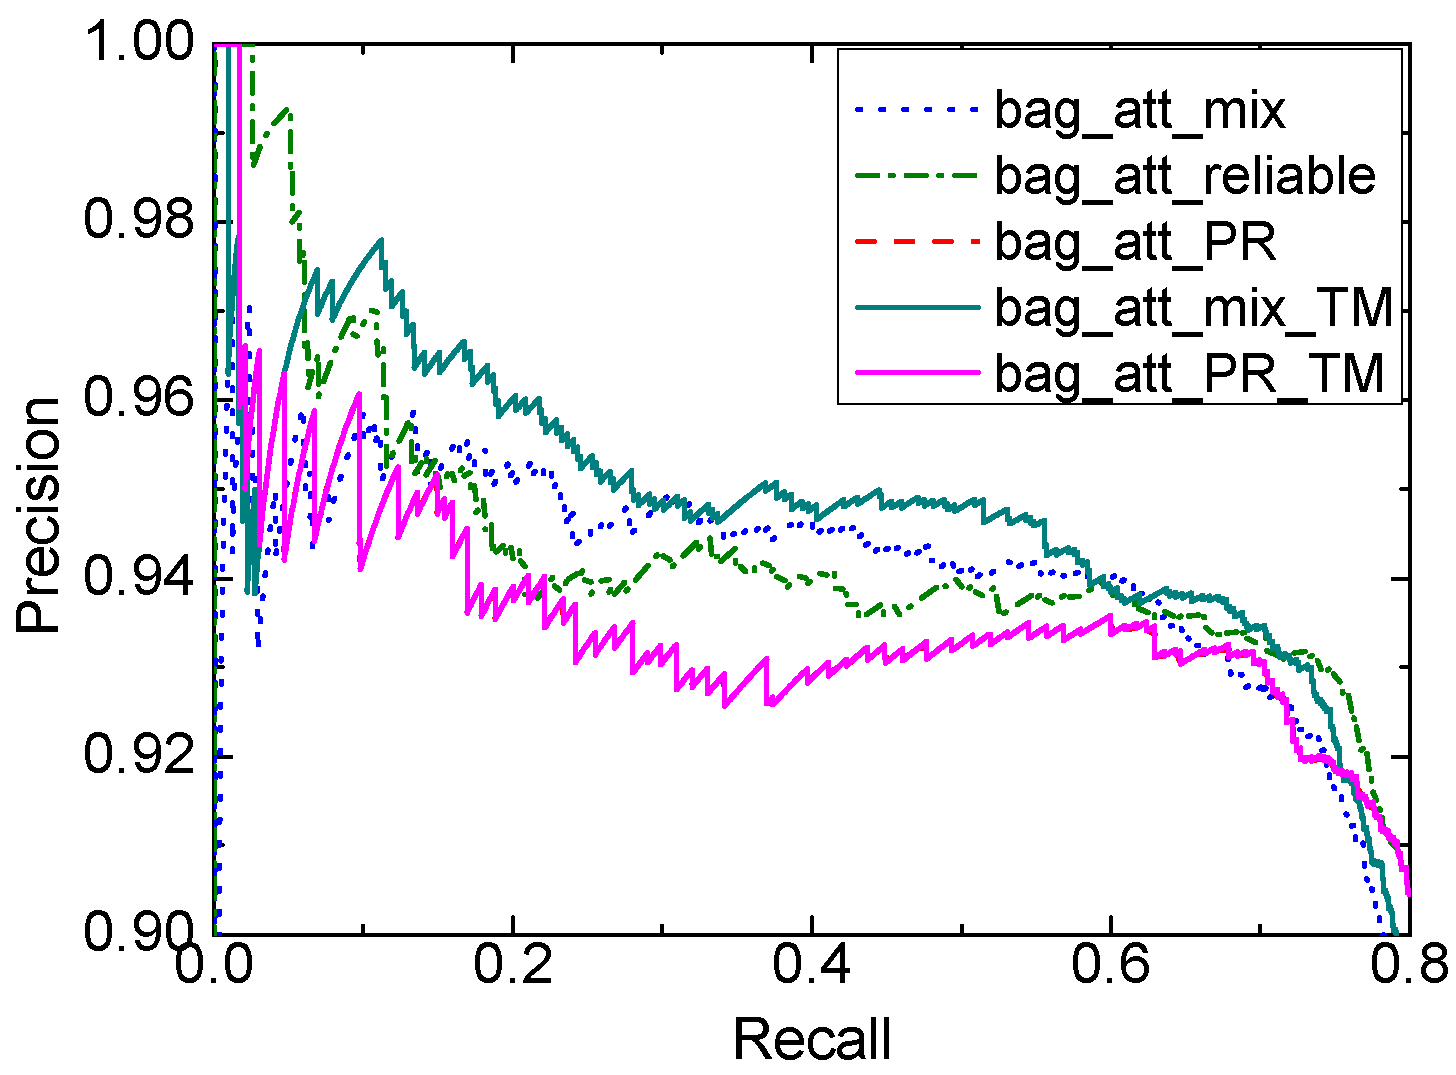
\includegraphics[width=0.48\textwidth]{figures/bag_avg_exp_overall.pdf}
\label{fig: bag_avg_luo}
}
\caption{Bag Level Results on TimeRE}
\label{fig: results_on_luo}
\end{figure*}

\subsection{Performances on \TimeRE} \label{sec:results_in_TimeRE}

\paragraph{Sentence Level Models}
The results of sentence level models on \TimeRE are shown in Figure \ref{fig:
sent_luo}. We can see that mixing all subsets together (\texttt{sent\_mix})
gives the worst result. The performance of this strategey is significantly
worse than using the reliable subset only (\texttt{sent\_reliable}). This
suggests the noisy nature of the training data obtained through \DS and
properly dealing with the noise is the key for \DS to be adopted at a wider
scale. When getting help from our transition matrix during training, the
model (\texttt{sent\_mix\_TM}) significantly improves (\texttt{sent\_mix}),
delivering the same level of performance as (\texttt{sent\_reliable}) in most
cases. This suggests that our transition matrix can help to mitigate the bad influence of noisy training instances.


Let us consider the \texttt{PR} scenario where one can build a curriculum by first training on the
reliable subset and then gradually moving to the space with both reliable and less
reliable subsets. In this case, the curriculum learning based model
(\texttt{sent\_PR}) even  outperforms \emph{sent\_reliable} significantly \red{(F: does \texttt{sent\_PR} have help from other components? e.g., TM?) } \orange{No},
indicating that the curriculum learning framework not only reduces the effect
of noise, but also helps the model learns from noisy data. When applying the
transition matrix approach into this curriculum learning framework using one reliable
subset and \orange{one unreliable subset generated by mixing the two less reliable subsets, our model (\emph{sent\_PR\_seg2\_TM})
further improves \emph{sent\_PR} by  %exploring the prior knowledge about data quality and
enabling it to use transition matrix to model the noise}
%enabling the transition matrix approach to control the noise at different levels during different curriculums. }
% \todo{ZW: Have no idea of what this sentence is talking about. \textbf{I have rephrased it}.}
(\orange{I further rephrased this sentence.})
\orange{It is not surprising that when we use all three subsets separately,}
our model (\emph{sent\_PR\_TM}) significantly outperforms all
other models by a large margin\footnote{We will use all three subsets for all
\emph{\_PR} settings in the rest of the experiments.}. \todo{ZW: I
rephrase some of the sentences, but I still think this paragraph needs to be
written.}


\paragraph{Bag Level Models}
In this experiment, we first look at the performance of the bag level models with attention aggregation. The results are shown in Figure \ref{fig: bag_att_luo}.
Consider a comparison between the  model trained on the reliable subset only (\texttt{bag\_att\_reliable}) and the model trained on the mixed dataset (\texttt{bag\_att\_mix}).
In contrast to the sentence level cases, \texttt{bag\_att\_mix} outperforms \texttt{bag\_att\_reliable} by a large margin. This is due to the fact that \texttt{bag\_att\_mix} has taken the noise within the bag into consideration through the attention aggregation mechanism, which can be seen as a denoising step within the bag.
This may also be the reason that when we introduce either our transition matrix approach \red{(\texttt{bag\_att\_mix\_TM})}  or the curriculum of using the reliable data first (\texttt{bag\_att\_PR}) into the bad level model, the improvement compared to \texttt{bag\_att\_mix}  is not as significant as in the sentence level.
However, when we utilize our transition matrix approach to model the noise with the curriculum of using the reliable data first (\texttt{bag\_att\_PR\_TM}), the performance gets further improved. This is especially in the high precision part compared to \texttt{bag\_att\_PR}.
We also note that the bag level's \textit{at-least-one} assumption does not always hold, and there are still false negative and false positive problems. Therefore, we can see that using our transition matrix approach with or without prior knowledge of data quality, i.e., \texttt{bag\_att\_mix\_TM}  and \texttt{bag\_att\_PR\_TM}, both improve the performance, and \texttt{bag\_att\_PR\_TM} performs slightly better.

%\paragraph{Bag Level Average Aggregation Models}
The results of the bag level models with average aggregation is shown in Figure \ref{fig: bag_avg_luo}. The relative ranking of various settings is similar to those with the attention aggregation.
One of the notable differences is that both \texttt{bag\_avg\_PR} and \texttt{bag\_avg\_mix\_TM} improve \texttt{bag\_avg\_mix} with larger margins compared to that in the attention aggregation setting. The reasons may be that the average aggregation mechanism is not as good as the attention aggregation one in terms of denoising ability, which leaves more space for our transition matrix approach or curriculum learning with prior knolwdege of data quality to improve.
\orange{We can also see that \texttt{bag\_avg\_reliable} performs best in the very-low-recall region but worst in general.
This is because that it ranks highly the sentences expressing relation \emph{birth-date} and \emph{death-date} which are the simplest and the most common relations in the dataset. However, due to the less amout of data, this model performs worse in other relations and thus generates the worst results in general.}
% Therefore, this shows that training only on the reliable data leads the model to use the most common patterns with high confidence, but the less amount of data makes it performs worse in general.
%\red{why (\texttt{bag\_avg\_reliable}) performs so much better than all others in the very high precision stage ($recall<0.05$)?????????}
%\orange{Another prominent difference lies in the performance drop of \emph{bag\_avg\_PR\_TM} in the low-recall area ($recall<0.15$). With manual investigation, we find that this is caused by some high ranking of false negative data}
%However, since  denoising ability is not as good as attention aggregation, adding unreliable data gradually (\emph{bag\_avg\_currd}) improves the model performance here. We can also see that the transition matrix improves the average aggregation models more significantly than the attention aggregation models.
 %Note that due to the inferior denoising ability of average aggregation, the unhandled sentence level noise may further propagates to bag level, which gives the transition matrix more chance to help model the noise.

\begin{figure}[htbp]
\begin{center}
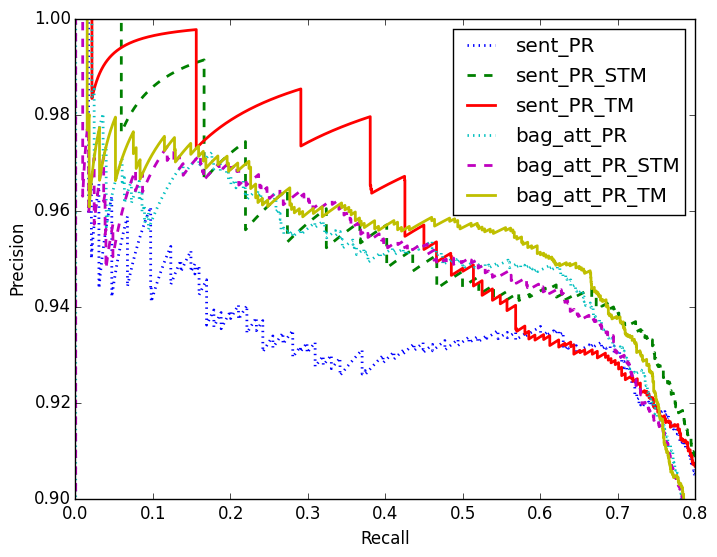
\includegraphics[width=0.9\linewidth]{figures/single_cmp_exp_overall.png}
\caption{Single TM and Dynamic TM}
\label{fig: cmp_single_dynamic}
\end{center}
\end{figure}

\paragraph{Global v.s. Dynamic Transition Matrix}
We also compare our dynamic transition matrix method with the global transition matrix method.
Specifically, instead of dynamically generating a transition matrix for each datum, the global transition matrix method use a single transition matrix for all the traning data. First, we initialize an identity matrix $\mathbf{T}'\in\mathbb{R}^{k\times k}$ where $k$ is the number of relations (including \orange{\emph{no\_relation}, (unify the notation)}), then the global transition matrix is calculated with row-wise softmax:
\begin{equation}
\label{shared_mat}
T_{ij} = \frac{e^{T'_{ij}}}{\sum_{j=1}^{k}{e^{T'_{ij}}}}
\end{equation}
where $T_{ij}$ and $T'_{ij}$ are the elements in the $i^{th}$ row and $j^{th}$ column of $\mathbf{T}$ and $\mathbf{T}'$. The element values of matrix $\mathbf{T}'$ are also updated via backpropagation during training.
The results are shown in Figure \ref{fig: cmp_single_dynamic}.
We can see that using only a global transition matrix (\texttt{\_GTM}) is also beneficial and it improves both \texttt{sent\_PR} and \texttt{bag\_att\_PR}. However, since the global transition matrix only captures global noise pattern and will therefore have incorrect behavior when the data is reliable, it performs worse than our dynamic transition matrix methods (\texttt{\_TM}).

\begin{figure}[t!]
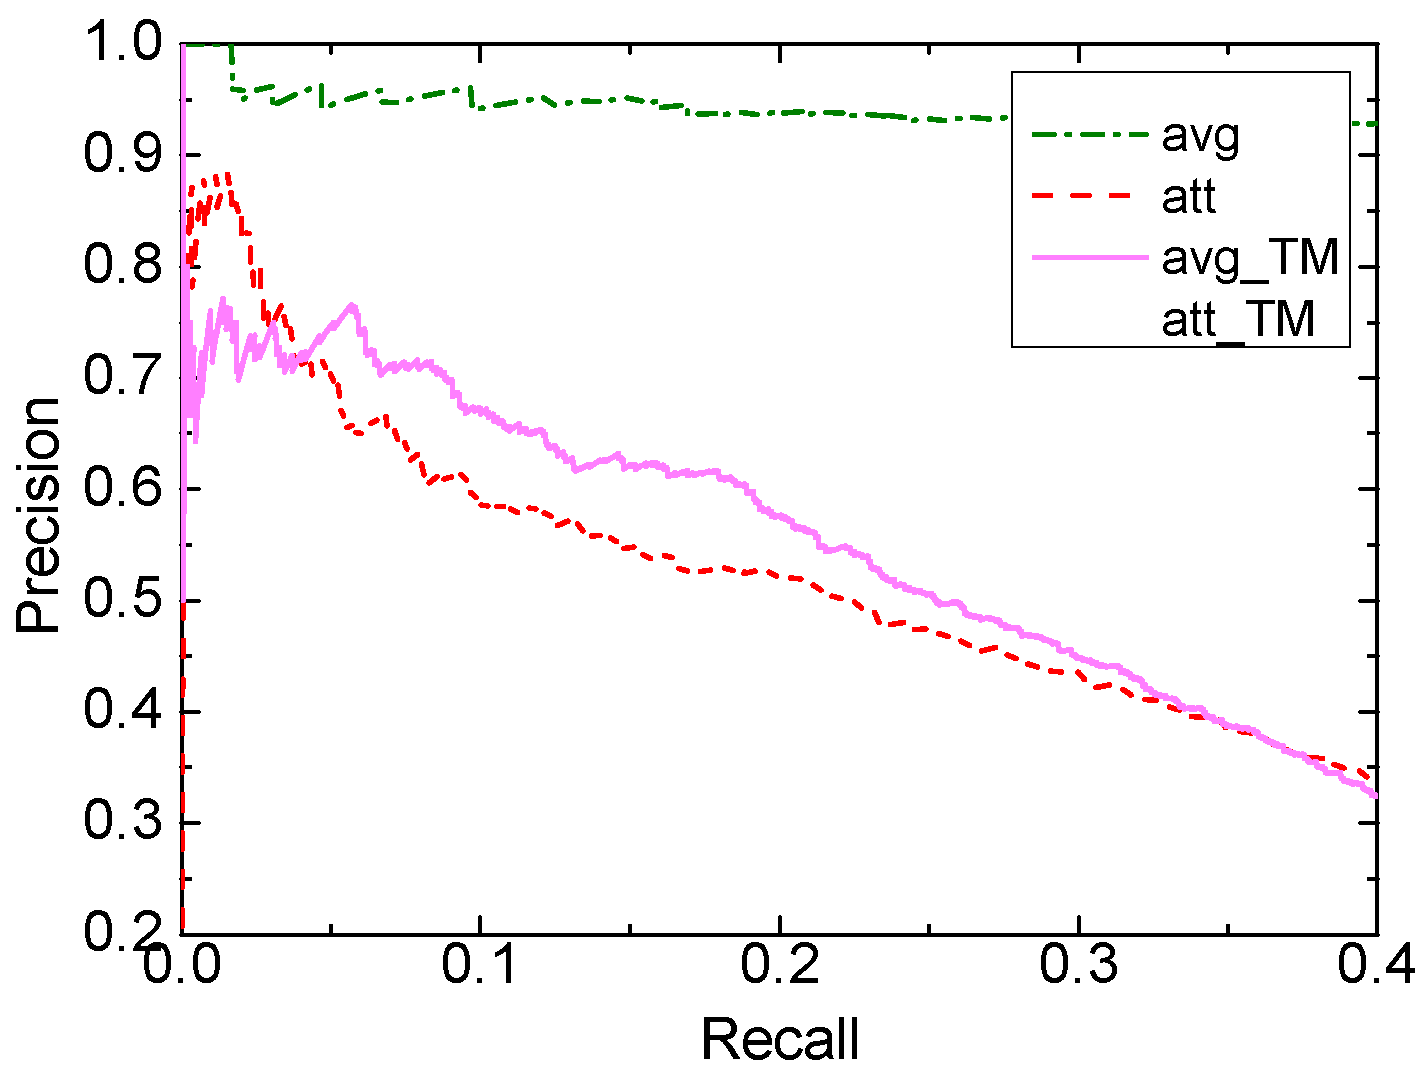
\includegraphics[width=0.48\textwidth]{figures/re_att_avg_cmp_exp.pdf}
\caption{Results on Dataset of Riedel et.al.}
\label{fig: Riedel_res}
\end{figure}

\subsection{Performance on \EntityRE}
We also conduct experiments on the \EntityRE dataset, where we can evaluate our bag level models only. \todo{ZW: Why bag-level models only? We need a an answer! } \blue{F: I put a sentence in data preparation.}
We  implemented the average aggregation method (\texttt{avg}), and the attention aggregation method (\texttt{att}) proposed by \cite{lin2016neural} as well as their corresponding transition matrix versions (\texttt{avg\_TM} and \texttt{att\_TM}). As we can see in Figure \ref{fig: Riedel_res},  due to the inferior denoising ability of the average aggregation component, \texttt{avg} performs worst among all those models. %Similar to the trends on the TimeRE data, when
\red{what should we say about this figure????}
When we inject our transition matrix approach into both \emph{avg} and \emph{att}, the resulting two  models, both of which can  clearly outperform their basic extraction models.
%
%since the unhandled sentence level noise propagates to the bag level, which makes the bag level noise become more severe, the transition matrix has more chance to model the noise. Therefore, the \emph{avg\_TM} model clearly outperforms the \emph{avg} model.
\orange{Again, because the attention aggregation model already has good ability in reducing the impact of sentence level noise and the bag level noise is less significant than the sentence level noise, the improvement of our transition matrix model is limited, which only improves the model on the low recall part.}
%Since
%Note that the low recall part corresponds to high precision, which is more useful than the rest of the extraction results in practice. Therefore, our transition matrix method is also useful in this situation.

\subsection{Summary}
\todo{ZW: This section is incredibly complex. I suggest to have a summary section to highlight the take away messages.} 